\documentclass[10pt,a4j]{jsarticle}

\usepackage[dvipdfmx]{hyperref}
\usepackage{color}
\usepackage{listings,jlisting}
\usepackage[top=5truemm,bottom=13truemm,left=8truemm,right=8truemm]{geometry}
\usepackage[dvipdfmx]{graphicx}
\usepackage{wrapfig}

\lstset{
	language={C++},
	backgroundcolor={\color[gray]{.85}},
	frame={shadowbox},
	commentstyle={\color[rgb]{0,0.5,0}},
	keywordstyle={\color[rgb]{1,0,0}},
	stringstyle={\color[rgb]{0,0,1}},
	breaklines=true,
	lineskip=-0.6zw,
	basicstyle={\ttfamily},
	tabsize=4,
}

\renewcommand{\baselinestretch}{0.9}

\title{\vspace{-1.0cm}OSが動作するx86エミュレータの開発}
\author{坂本優太}
\date{}

\begin{document}
\maketitle
\vspace{-1.0cm}

\section{背景}
\cite[30日でできる! OS自作入門]{30days-osdev}という本をきっかけにプログラミングを初めた僕は,
2016年のセキュリティ・キャンプ全国大会に参加し,よりコンピュータの仕組みに興味を持つようになった.
その後,僕は\cite[自作エミュレータで学ぶx86アーキテクチャ]{learn-x86-by-emu}を読んだことで,
\cite{30days-osdev}では自作OSの動作確認のために使っているだけだったエミュレータというプログラムの仕組みにも興味を持つようになった.

エミュレータとは,コンピュータの動作をエミュレート,つまり模倣するプログラムのことで,代表的なものとしては
QEMU\footnote{Fabrice Bellardが中心となって開発しているオープンソースのエミュレータ.
動的バイナリ変換(Dynamic Binary Translation)などの機能を持ち,高速に動作するのが特徴.}
やBochs\footnote{オープンソースのPC/AT互換機のエミュレータ.}などがある.
これらのエミュレータはコンピュータをほぼ正確に模倣するため,
WindowsやLinuxなどの主要なOSや,「はりぼてOS」\footnote{\cite{30days-osdev}で作る小さなOS.}を動かすことができる.
このように,仮想的なコンピュータ上でソフトウェアを動作させることを仮想化といい,
これらの技術は最近ではOSや別アーキテクチャのソフトウェアの動作確認だけでなく,
作業環境の分離などにも用いられる一般的な技術となっている\footnote{ただし,これは正確には準仮想化と呼ばれるものの方が多い.}.

しかし,\cite{learn-x86-by-emu}で作るエミュレータはとても小さく機能もとても少ないものであり,
WindowsやLinuxなどのOSを動かすことができないのはもちろん,「はりぼてOS」のような小さなOSも動かすことはできなかった.
そこで,これらのOSを動かすために必要なエミュレータの機能を考え,独自のエミュレータを開発を初めた.
ただし,WindowsやLinuxのような大きなOSを動かすためにはとても多くの機能を実装する必要があるため,
あくまで「はりぼてOS」を動かすことを目標とした.

\section{成果の具体的な内容}

\subsection{エミュレータの設計}
% コード示してから本のエミュとの相違点説明の方が分かりやすい・書きやすいかも?

\cite{learn-x86-by-emu}のエミュレータはCで実装されていた.
しかし,これを改良していこうとするとコードが煩雑になってしまう上,
改良するのではなく1から作り直すことで既に実装されている部分についても十分に理解したいと考えた.
そこで,多少は使い慣れていたC++を使い,
Cでのコードを参考にしつつも1から実装することにした\footnote{このときのリポジトリは\url{https://github.com/sk2sat/vm}}.

C++によるエミュレータの実装の基本的な部分はソースコード\ref{impl-emu-base}のようになった.
\begin{lstlisting}[caption=エミュレータの基本的な実装,label=impl-emu-base]
typedef union {
	uint32_t reg32;
	uint16_t reg16; // 下位16bit
	struct {
		uint8_t low8, high8;
	};
} Register32; // 32bit register

class Emulator {
	public:
		Register32 CR[5], eflags, eip, reg[8];	// レジスタ
		uint8_t *memory;			// メモリ
	private:
		int bite_mode, memory_size;
}

typedef void instruction_func_t(Emulator *emu); // 1つの命令に対応する関数の型
instruction_func_t* instruction16[256];
instruction_func_t* instruction32[256];
\end{lstlisting}
Emulatorクラスは,コンピュータを構成する要素であるCPUやメモリを1つにまとめたもので,
このクラスがエミュレータの本体となる.
Register32は32bit長のレジスタを表す共用体で,
メンバを使って下位の8,16bitの領域へのアクセスが行いやすくなっている.
これは実際のレジスタもそのようなアクセスがあるためで,
例えばEAXというレジスタは下位16bitがAX,そのうち上位8bitがAH,下位8bitがALという名前のレジスタとして扱われる.
また,メモリはuint8\_t型の並んだメモリ領域として表現した.

こうすると後は,この仮想的なメモリ上に実行するプログラムを置いて,
実行するアドレスにある機械語を読み込み(fetch),意味を解析(decode)して実行する,
という一連の処理を無限ループすればエミュレータになる.
ここで,実行するアドレスはプログラム・カウンタという専用のレジスタの値を使うことになっている.
x86ではEIPがこれに相当するため,このプログラムでいうとmemory[eip.reg32]が実行される機械語の最初のバイトになる.

実行される1つ1つの機械語命令はそれぞれ1つの関数で表現されており,
Emulatorクラスはこれらの命令のポインタの配列を持っている.
こうしておくことで,オペコードnの命令を実行する時はinstruction[n]が指す関数を実行すればよく,
実装を分かりやすくすることができる.
これは\cite{learn-x86-by-emu}の実装を元にしたものだ.
しかし,本の実装では命令は32bitモードのみなので,
複数の動作モードに対応するため,16bitと32bitそれぞれに関数ポインタ配列を用意して,
動作モードによって使用する配列を分岐するという実装になっている.

\subsection{ディスプレイの実装}
QEMUやBochsなどのエミュレータでは,ディスプレイのエミュレートをすることもできる.
エミュレータには必ずしもディスプレイのエミュレートが必要という訳ではない.
しかし,動作目標の「はりぼてOS」は比較的GUIの比重が大きい他,
単純に「はりぼてOS」のUIが自分のエミュレータで見られると嬉しいと思ったため,実装することにした.

ディスプレイは,指定した色で発光するピクセルが解像度の分だけ並んでいるデバイスであり,
描画はそれぞれの座標への色の指定という形で行われている.
この座標と色の設定は,実際にはVRAMというメモリ領域への書き込みによって実現されている.

このVRAMでは1ピクセルに相当するのは1byteとなっている.
これではRGBで色を指定することができないので,ここに書き込むデータはRGBのような色データではなく,
パレットという外部装置に事前に設定しておいた色の番号ということになっている.

これらをエミュレートするため,
\begin{itemize}
	\item 外部装置へのアクセス
	\item パレット
	\item VRAMのデータからRGBデータを生成
	\item RGBデータをウィンドウに表示
\end{itemize}
の実装を行った.

x86では,外部装置へのアクセスはin/out命令で行われる.
これは,デバイスの基本クラスを作り,
in/out命令が実行されると対応するデバイスのクラスの関数が呼ばれるようにすることで表現した.
ディスプレイは1つのデバイスクラスとしてデバイスの基本クラスを継承して作り,
RGBのテーブルとして表現したパレットをout命令で設定できるようにした.

VRAMのデータから実際に描画されるRGBのデータを生成するのは,
画面上の全ての座標においてVRAMから読み取った色番号に対応する色データをパレットから取得して設定することで実装した.

\begin{lstlisting}
unsigned char* Display::Draw(){
	for(int x=0;x<scrnx;x++){
		for(int y=0;y<scrny;y++){
			int i = y*scrnx + x;
			char n= vram[i]; // (x,y)の色番号
			img[i*3  ] = palette[n*3  ];
			img[i*3+1] = palette[n*3+1];
			img[i*3+2] = palette[n*3+2];
		}
	}
	return img;
}
\end{lstlisting}

生成したRGBデータをウィンドウに表示する部分は,
オープンソースでマルチプラットフォーム対応のGUIライブラリであるfreeglutを使用した.

\subsection{テスト環境の整備\label{impl-test-env}}
% haribote-os
% make runでバージョン指定してテストできるようにした

「はりぼてOS」を動作させることが最終的な目標ではあったが,
初めから「はりぼてOS」の最終バージョンを動かそうとしてしまうと,
どこまでは動作していて,どこからが動作していないのか,
どこにバグが残っているのかという問題を切り分けて考えることがとても難しくなってしまう.
そこで,エミュレータのテストを行うためのバイナリについても自分で整備することにした.

\cite{30days-osdev}では,本文中で「はりぼてOS」の開発がインクリメンタルに進められていく.
そのため,「はりぼてOS」は初めの方ほど機能が少ないためエミュレートもしやすく,
段々と機能が実装されていくにつれてエミュレータに要求される機能も増えていく.
また,「はりぼてOS」は章・節と対応した,"harib01c"というようなバージョン名が付けられている.
僕はこれを利用して,特定のバージョンの「はりぼてOS」をビルドするための環境を作り,
それを使ってエミュレータのテストをすることで,
自分のエミュレータで動作する「はりぼてOS」のバージョンを少しずつ上げていく開発スタイルを確立した.

このために作ったのがharibote-osというリポジトリ\footnote{\url{https://github.com/sk2sat/haribote-os}}で,
これを使うと,「はりぼてOS」のバージョンごとに対応したブランチやタグを選択して"make"コマンドを実行するだけで,
指定のバージョンの「はりぼてOS」のバイナリを生成することができる.

これにより,エミュレータ\footnote{\url{https://github.com/sk2sat/emu}}の方のリポジトリで
"make run HARIB\_VER=harib01c"のようにして「はりぼてOS」のバージョンを指定したテストが行えるようになった.

\subsection{セグメンテーションの実装\label{impl-segmentation}}
x86には,「セグメンテーション」という機能がある.
これはメモリ管理機能
\footnote{メモリ管理機能にはセグメンテーションの他にページングというものもあり,現在ではこちらの方が主流だが,「はりぼてOS」では使用されていないため実装はしなかった.}
の1つで,メモリを用途ごとに分割する役割と,アクセス制御を行う役割がある.
セグメンテーションでは,メモリ領域をセグメントという単位で分割する.
そして,それぞれのセグメントの属性を設定することで,メモリ領域の管理やアクセス制御を行うことができる.

メモリ領域をセグメントに分けることによる最も大きなメリットは,
物理アドレスを気にしてプログラミングする必要がなくなる,という点にある.
例えば,あるセグメントの開始アドレスが物理アドレスで0x10000とする.
このとき,このセグメントをデータ用のセグメントと指定した上で,
0x00というアドレスにあるデータを取得する命令を実行すると,
CPUのアドレス変換という機能\footnote{正確には,CPU内のMMUがこのアドレス変換を行っている.}により,
実際には物理アドレスで0x10000にあるデータが取得される.

このようなアドレス変換の実装は,ソースコード\ref{L2P}のようになった.
\begin{lstlisting}[caption=論理アドレスの物理アドレスへの変換,label=L2P]
uint32_t Emulator::L2P(const x86::SRegister *sreg, const uint32_t &addr){
	if(!IsProtected())
		return (sreg->reg16 * 16) + addr; // real mode
	Descriptor desc;
	desc.low32 = GET_MEM32(GDTR.base+(sreg->index*8));
	desc.high32= GET_MEM32(GDTR.base+(sreg->index*8)+4);
	return addr + desc.GetBase();
}
\end{lstlisting}
この関数は,セグメントレジスタと論理アドレスを引数にとり,物理アドレスを返す.
セグメントレジスタというのは,どのセグメントを使うのかを指定するためのレジスタで,
その用途によって,コードセグメント用のCS,データセグメント用のDSなどのものがあある.

リアルモードにおいては,セグメンテーションはとても単純で,
物理アドレスはセグメントレジスタの値に16をかけたものに論理アドレスを加算したものになる.

一方,プロテクトモードではセグメントの開始アドレス,サイズ,属性を自由に設定できるようになっている.
この属性というのは,
データ用なのか,実行可能なのか,実行可能なら16,32bitのどちらのモードで実行するのか,どの特権レベルからアクセスできるのか,
といったものを設定できる.
このような設定ができるのがプロテクトモードが「プロテクト」モードたる所以でもある.

では,このようなセグメントの情報はどのように設定するのかというと,
とてもレジスタのような小さな記憶領域には保存できないため,
GDTと呼ばれるメモリ領域に保存する.
GDTはGlobal Descripto Tableの略で,
1つのセグメントの属性などをまとめたDescriptorという構造体が連続して並んでいる領域のことだ.
そして,このGDT内でのDescriptorの番号をセグメントレジスタに入れることで,セグメントを指定することができる.

このため,Descriptorを表す構造体を作り,
GDTの開始アドレスにセグメントレジスタの値の分を足したアドレスからデータを取得してDescriptorに代入し,
そこからセグメントの開始アドレスを取得して論理アドレスに足す,という実装になった.

上記のようにして,セグメンテーションのアドレス変換の部分は実装することができた.
ただし,アクセス制御を行う部分はまだCPUの特権レベルなどが存在しないためこれから実装することになる.
また,セグメンテーションは簡単な使い方こそ知っていたもののその詳細な動作や仕様はよく分かっていなかったため,
実装にあたっては\cite[はじめて読む486]{read-486}と\cite[SDM]{SDM}が大いに参考になった.

\begin{wrapfigure}[10]{r}[1mm]{85mm}
	\vspace{-7mm}
	\caption{自作エミュレータ上で「はりぼてOS」が起動メッセージを表示するところまで完全に動作するようになった.}
	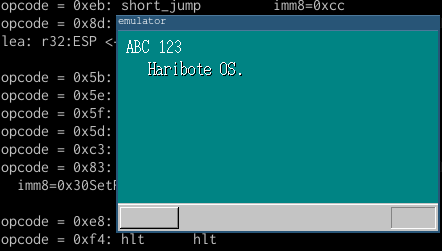
\includegraphics[width=85mm]{emu.png}
\end{wrapfigure}

これにより,「はりぼてOS」のブートローダが起動してから,「はりぼてOS」本体をメモリに転送し,
プロテクトモードに移行し,セグメントを設定,C言語で書かれたメイン関数が実行され,起動メッセージが表示される,
というところまでを自分のエミュレータで完全に動作させることができるようになった.

\section{サイボウズ・ラボユースでの活動}
%・vmからemuに
%・SDMたべる
%・ログの出力

僕はこのx86エミュレータの開発を完全に趣味で行っていた.
そんなとき,2017年の2月に東京で開催されたOSC
\footnote{Open Source Conference Tokyo/Springのこと.}
でサイボウズ・ラボユースという学生支援制度を\cite{30days-osdev}の著者の川合さんに紹介していただいた.
これはサイボウズ・ラボが実施しているもので,メンターの指導と奨励金の支給を受けつつOSSを開発できる制度である.
僕はx86エミュレータの開発をテーマにこの制度に申し込み,書類選考と面接を経て
第7期サイボウズ・ラボユースにラボユース研究生
\footnote{この制度には奨励金の有無のみが異なるラボユース生とラボユース研究生の2つのコースがある.僕はラボユース研究生としては初の採択だったようだ.}として採択された.

ラボユースの期間中,実際に出社できたのは夏休みの間の数回だけのことだったため,
開発は基本的に自宅で行い,メンターの光成さんからリモートでコードレビューを頂いたり,
\cite{read-486}や\cite{effective-cpp}などの書籍を貸して頂いて参考にしたり,というのがラボユースでの主な活動となった.
この他にも,ラボユース内でのC++勉強会や,同期のラボユース生の方との交流などができ,とても多くの学びが得られた.

\ref{impl-test-env}と\ref{impl-segmentation}はラボユース期間中の主な成果である.

2018年3月,「第7期サイボウズ・ラボユース成果発表会」\footnote{\url{https://blog.cybozu.io/entry/2018/04/05/080000}}で成果発表を行い,
僕はサイボウズ・ラボユース研究生を卒業した.

\section{今後の方針}
%・新たな実装
%・実装の見通しの悪さを改善
%・ラムダ式

現在,「はりぼてOS」の全てのバージョンを動作させることを目標として,新たなx86エミュレータを1から開発している.
改良するのではなく作り直す理由は,開発してきたエミュレータの実装は見通しが悪いため,
デバッグや改良にかかる労力が大きすぎると判断したからだ.
新たな実装は同一リポジトリのv2ブランチ\footnote{\url{https://github.com/sk2sat/emu/tree/v2}}で行っている.

v2の開発では,設計の見通しの良さ\footnote{"数ヶ月後に見直しても難なく読める"ことが目標だ.}と,
実行中のメッセージの分かりやすさをとても重視している.
また,実装にはC++の最新の規格であるC++17を用いている.

v2での最も大きな変更点は,すべての命令の実装にC++のラムダ式を用いていることだ.
これにより,ソースコード\ref{use-lamda}のように,
x86の命令を関数型マクロを使ってとても見た目に分かりやすく実装することができるようになった.

\begin{lstlisting}[caption=ラムダ式を使った命令の実装の一部,label=use-lamda]
#define INSN(opcode, insn, f, block) \
	name[opcode] = #insn; \
	flag[opcode] = f; \
	func[op] = [](CPU &cpu, std::shared_ptr<Memory> memory) block;

	// 命令の実装
	INSN(0x00, add_rm8_r8, ModRM,{ SET_RM8( ADD(GET_RM8(), GET_R8(REG_NUM)) ); });
	INSN(0x04, add_al_imm8,Imm8, { AL = ADD(AL, IMM8); });
	INSN(0x0c, or_al_imm8, Imm8, { AL = OR( AL, IMM8); });
\end{lstlisting}

%通常,エミュレータに求められるのは高速な動作や多くのCPUへの対応だが,
%多くのエミュレータがこれらを優先した結果,ソースコードの可読性を少なからず犠牲にしている側面があるように感じる.
%\footnote{QEMU}
%もちろん,これらの点を蔑ろにしてしまうととても実用には耐えないので,これは仕方のないことだ.
%しかし,\cite{learn-x86-by-emu}のように,コンピュータの仕組みを理解するためにエミュレータを
%そのため,初学者がエミュレータについて学ぼうとした時,参考になるのは書籍\cite{learn-x86-by-emu}ぐらいのも

\section{単独の成果か否か}
単独の成果である.
実装に当たっては書籍\cite{learn-x86-by-emu}のプログラムを参考にはしたものの,設計を変更し,機能も大幅に増えたオリジナルのプログラムとなっている.
設計・実装はすべて1人で行った.
ただし,サイボウズ・ラボユース採択期間中は,ラボユース内のC++勉強会に参加した他,メンターの方に絶版となっていた書籍\cite{read-486}を貸して頂いたり,数回コードレビューを頂いたりした.
コードレビューで指摘されたのはC++の書き方に関するものであり,これによる設計やロジックの変更は生じなかった.
\footnote{コードレビューによる変更は"[FIX] from code review"という一連のコミットで行われている.}

成果は全てGitHub上で公開している.
該当するリポジトリは以下の3つである.
\begin{itemize}
	\item \url{https://github.com/sk2sat/vm}			当初作っていたエミュレータ
	\item \url{https://github.com/sk2sat/emu}			ラボユース申し込み後に作り直したエミュレータ
	\item \url{https://github.com/sk2sat/haribote-os}	「はりぼてOS」実行テスト用のプロジェクト
\end{itemize}

\begin{thebibliography}{99}
	\bibitem{30days-osdev} 30日でできる! OS自作入門
	\bibitem{learn-x86-by-emu} 自作エミュレータで学ぶx86アーキテクチャ - コンピュータが動く仕組みを徹底理解!
	\bibitem{SDM} Intel® 64 and IA-32 Architectures Software Developer’s Manual vol 1,2,3,4
	\bibitem{read-486} はじめて読む486 - 32ビットコンピュータをやさしく語る
	\bibitem{effective-cpp} Effective C++ - プログラムとデザインを改良するための55項目
\end{thebibliography}

\end{document}
